\section{Transition Rule Dependencies}
\label{sec:sts-rules-overview}

Figure~\ref{fig:sts-rules-dependencies} shows all STS rules, the sub-rules they
use and possible dependencies. Each node in the graph represents one rule, the
top rule being $\mathsf{CHAINHEAD}$.\@ A straight arrow from one node to another
one represents a sub-rule relationship.

An arrow with a dotted line from one node to another represents a dependency in
the sense that the output of the target rule is an input to the source one,
either as part of the source state, the environment or the signal. These
dependencies are between sub-rules of a rule.

\begin{figure}[htp]
  \centering
  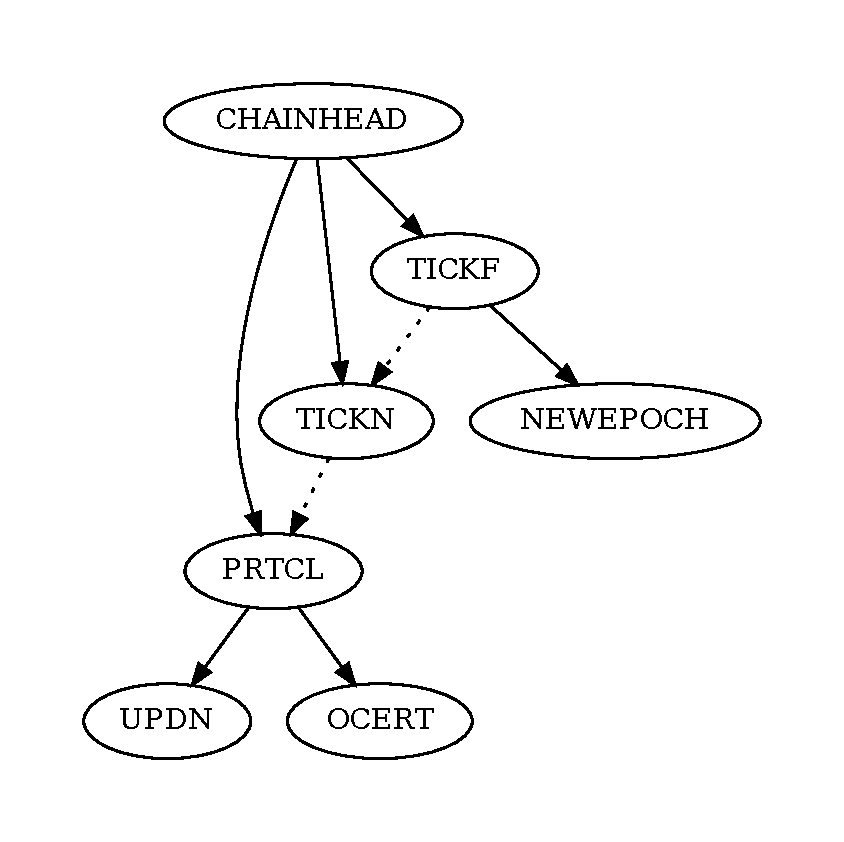
\includegraphics[width=\textwidth]{rules}
  \caption{STS Rules, Sub-Rules and Dependencies}
  \label{fig:sts-rules-dependencies}
\end{figure}

